\documentclass{report}
\usepackage{../header}

\newcommand{\rng}{\mathrm{range}}
\newcommand{\var}[1]{\mathrm{var}\left[{#1}\right]}
\newcommand{\cov}[1]{\mathrm{cov}\left[{#1}\right]}

\title{Элементы теории вероятностей. Обработка результатов экспериментов.}

\begin{document}
	\maketitle
	
\section{Вводные понятия}
Случайной величиной (с.в.) называется измеримая функция $X:\Omega\mapsto E$  из пространства возможных событий $\Omega$ в измеримое пространство $E$. Как правило, случайные величины вещественно-значны, т.е. $E=\mathbb{R}$.

Вероятность того, что $X$ примет значение из измеримого подмножества $S\subseteq E$
\[
P(X\in S) \equiv P(\{\omega\in\Omega| X(\omega)\in S\}).
\]
	
Если множество возможных событий счётно (то есть, каждому элементу $\omega\in\Omega$ можно сопоставить натуральное число $i\in\mathbb{N}$), то множество значений $\rng(X) = \{x_1, x_2, \dots, x_n\}$ тоже счётно. Такая с.в. называется \emph{дискретной}. Если же $\rng(X)$ не счётно, то $X$ -- непрерывная с.в.

\subsection{Операции с вероятностью}
\begin{itemize}
	\item логическое или ($\vee$): $P(A \vee B)  = P(A) + P(B)$ (Если $A$ и $B$ -- взаимно-исключающие события);
	\item логическое ($\wedge$): $P(A\wedge B) = P(A)\cdot P(B)$.
\end{itemize}
	
\section{Функция и плотность распределения случайной величины}
\subsection{Дискретная с.в.}

Пусть $X$ -- дискретная с.в. Тогда можно говорить о принятии величиной $X$ некоторого конкретного значения $x_i$, а следовательно 
\[
P(X\in\{x_i\}) \equiv P(X=x_i) = p_i.
\]
Функция $p: \mathbb{N}\mapsto\mathbb{R}$ называется \emph{распределением} вероятности дискретной величины.

Отсортируем значения $E = \{x_1, x_2,\dots, x_n\}$ и положим их на численную ось. Вероятность того, что $X$ примет любое из значений $x_i \leq x_j$ 
\[
P(X \leq x_j) \equiv F_X(x_j) = \sum_{i=1}^j p_i,
\]
и называется \emph{функцией распределения} (cumulative distribution function) с.в.  $X$.

\subsection{Непрерывная с.в.}
В случае непрерывной с.в., в качестве распределения вероятности используют \emph{плотность распределения} вероятности $f(x)$. Тогда, вероятность наблюдать величину $X$ в бесконечно-малом диапазоне значений $\rd x$:
\[
P(x\in (x_0, x_0+\rd x)) = f(x)\rd x,
\]
а в конечном диапазоне $[a, b]$, соответственно,
\[
P(X\in[a,b]) = \int_a^b f(x)\rd x.
\]

Очевидно, что определение функции распределения непрерывной с.в.
\[
F_X(x) = \int_{min\, E}^x f(\xi)\rd\xi,
\]
где $min\, E$ -- наименьший элемент множества $E$.

\begin{rmk}
	Из определения кумулятивного распределения непрерывной функции следует, что 
	\[
	P(x\in[a,b]) = F_X(b) - F_X(a).
	\]
\end{rmk}

\begin{figure}[h]
	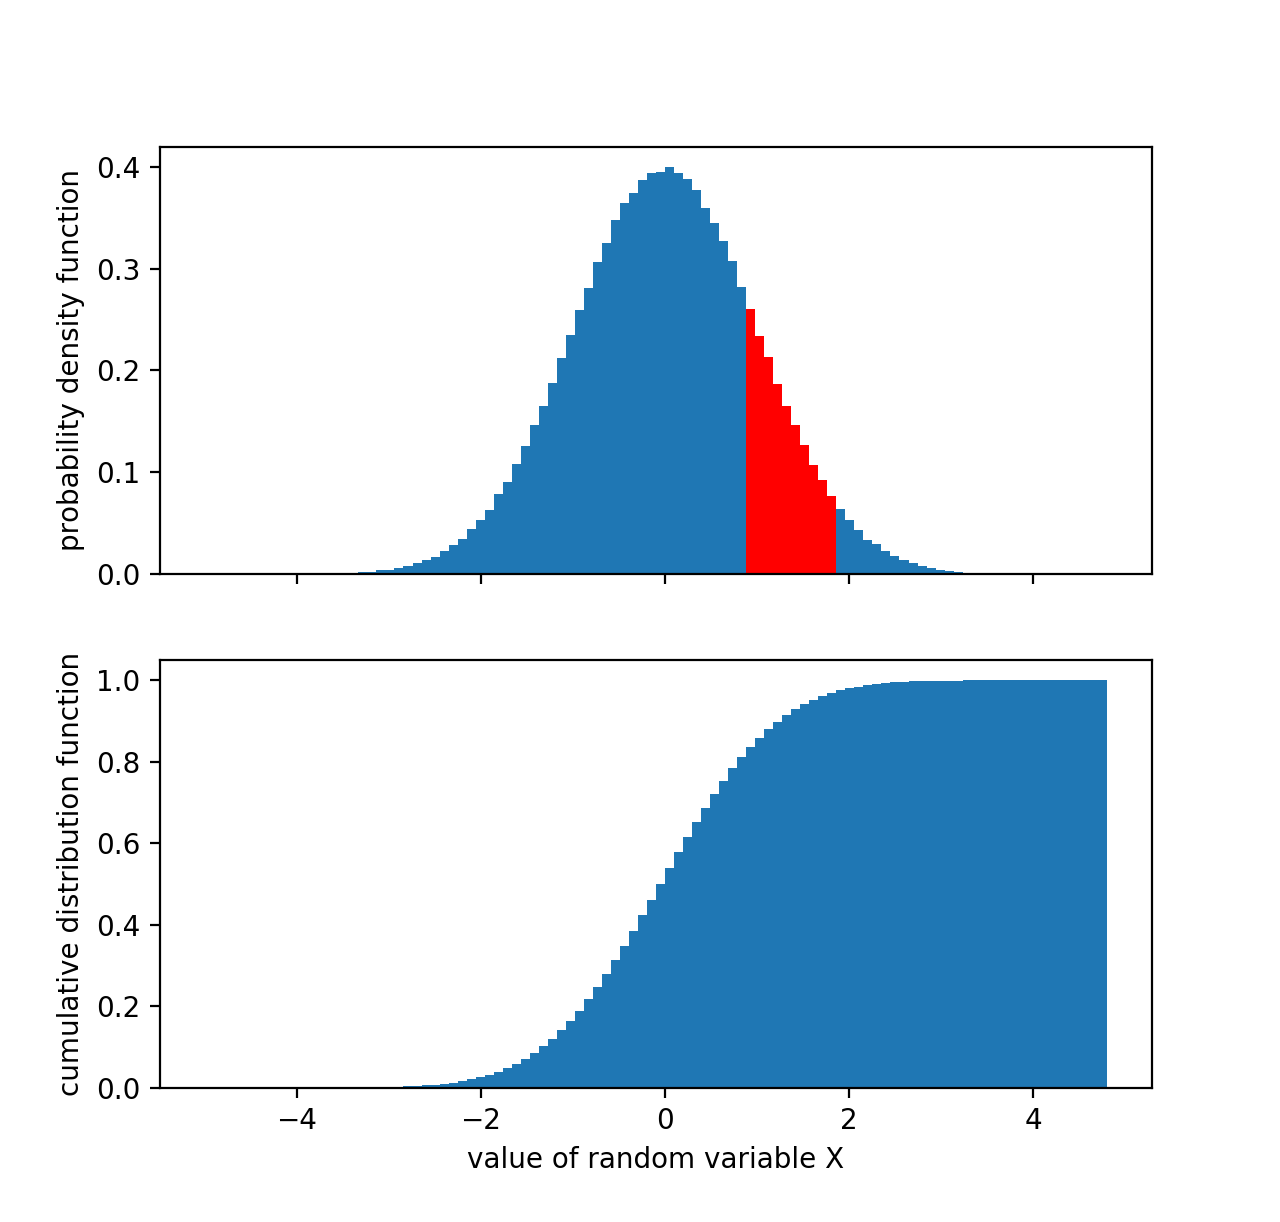
\includegraphics[width=\linewidth]{Normal_pdf_cdf}
	\caption{Плотность (верхняя панель) и функция (нижняя панель) распределения случайной величины $X\sim N(0, 1)$.\label{fig:continuous_rv_pdf_cdf}}
\end{figure}


\section{Числовые характеристики случайной величины}
\paragraph{Математическое ожидание}
\begin{itemize}
	\item \textbf{Дискретной} с.в.: $M[X] = \sum_i x_i p_i$.
	\item \textbf{Непрерывной} с.в.: $M[X] = \int_{-\infty}^{+\infty} xf(x)\rd x$.
\end{itemize}
\emph{Моментами} распределения называют математические ожидания следующих функций с.в. $X$:
\begin{align}
	\mu_1 &= M\left[X\right] \equiv m, \tag{матожидание}\\
	\mu_2 &= M\left[(X-m)^2\right] \equiv \sigma^2, \tag{дисперсия}\\
	\mu_3 &= M\left[(X-m)^3\right], \tag{асимметрия}\\
	\mu_4 &= M\left[(X-m)^4\right], \tag{kurtosis}
\end{align}
и так далее.

\begin{rmk}[Терминология]
	В русскоязычной литературе, то, что я обозвал kurtosis называют \emph{эксцесс}.
	Но, это не правильно, потому что есть kurtosis, и есть \emph{excess} kurtosis.
	Они отличаются следующим образом:
	\[
	\mu_4^e = \mu_4 - 3.
	\]
	Почему 3? 3 -- это куртосис нормального распределения. А вот \emph{эксцесс} куртосиса -- это на сколько
	куртосис распределения превосходит куртосис нормального распределения. Чем куртосис больше, тем острее распределение, и наоборот: чем он меньше, тем оно более пологое.
\end{rmk}

\begin{rmk}(Что характеризует куртосис?)
	По сути, куртосис говорит о вероятности наблюдения экстремального значения. \emph{Чем куртосис больше, тем более вероятно наблюдение экстремального значения} -- т.е. тем "толще" хвосты распределения. А поскольку интеграл распределения вероятности равен 1, чем толще хвост, тем уже середина, тем острее распределение. И наоборот. См. Рис.~\ref{fig:excess_kurtosis_pdfs}
\end{rmk}

\begin{rmk}
	Строго говоря, во всех формулах выше, вместо $m$ может стоять любое число $x_0$, включая ноль.
	Если $x_0=0$, то такие моменты называются \emph{начальными}; если $x_0 = M\left[ X\right]$, такие моменты называются \emph{центральными}. Последнее потому, что, для \emph{симметричного} распределения (например, нормального распределения $N(\mu, \sigma)$), матожидание является
	центральной точкой. При этом, для асимметричных распределений (например, $\chi^2$-распределения) это не так.
\end{rmk}

\begin{figure}[h]
	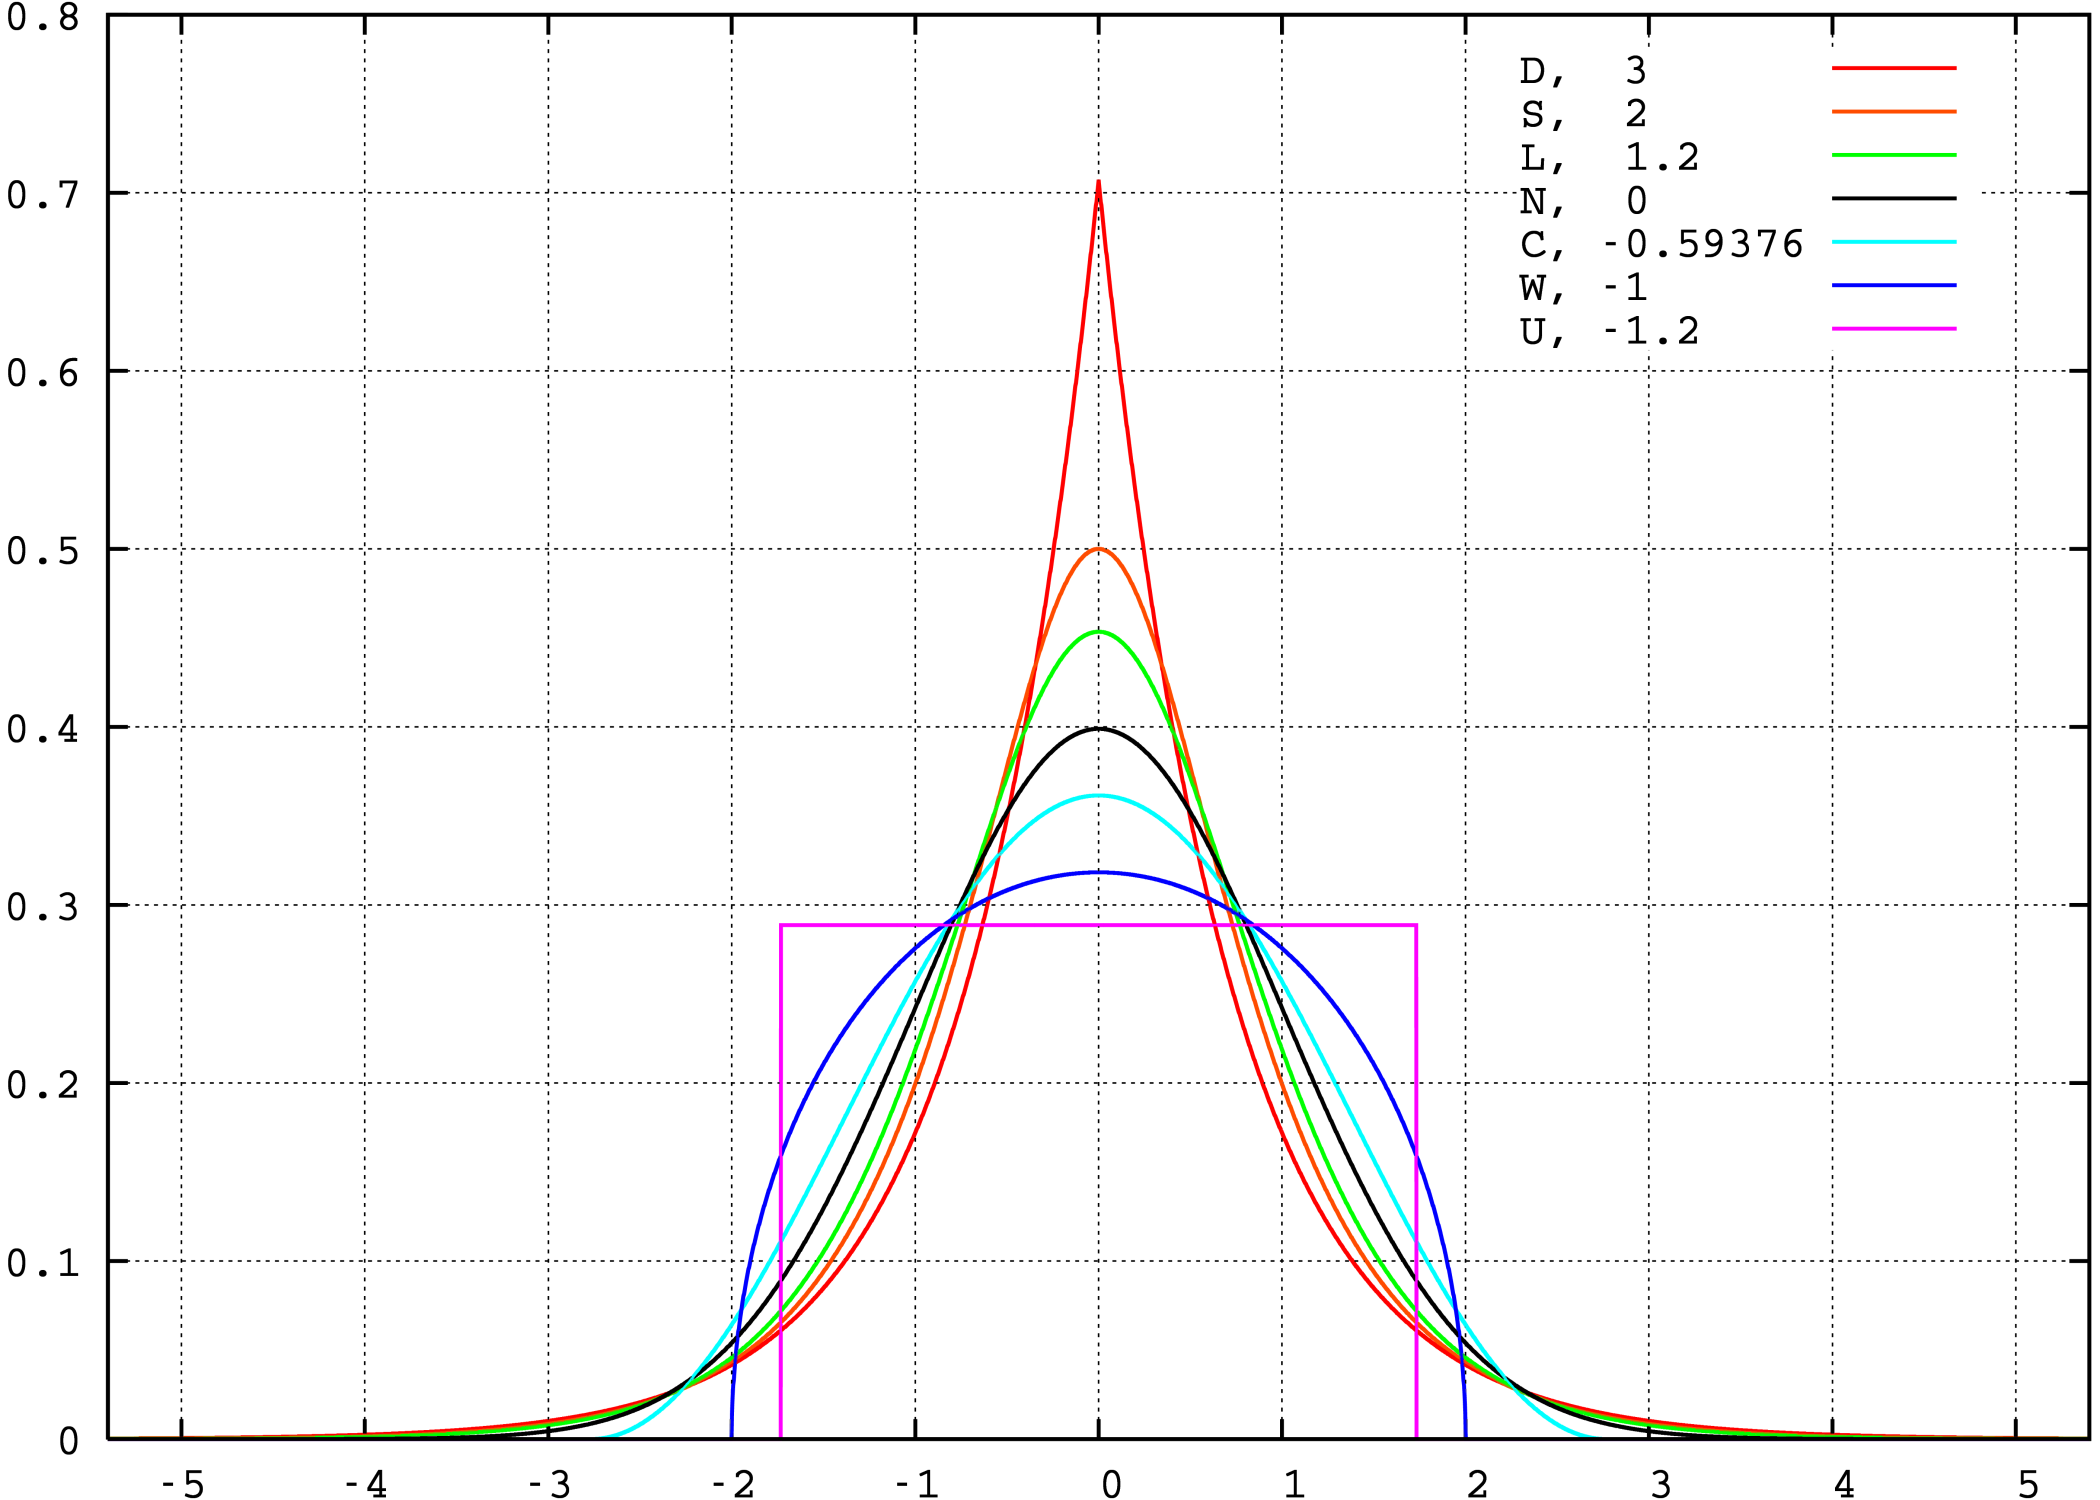
\includegraphics[width=\linewidth]{different_kurtosis_pdfs}
	\caption{Плотности распределения вероятности с различными значениямии эксцесса куртосиса (на легенде).\label{fig:excess_kurtosis_pdfs}}
\end{figure}

\begin{figure}[h]
	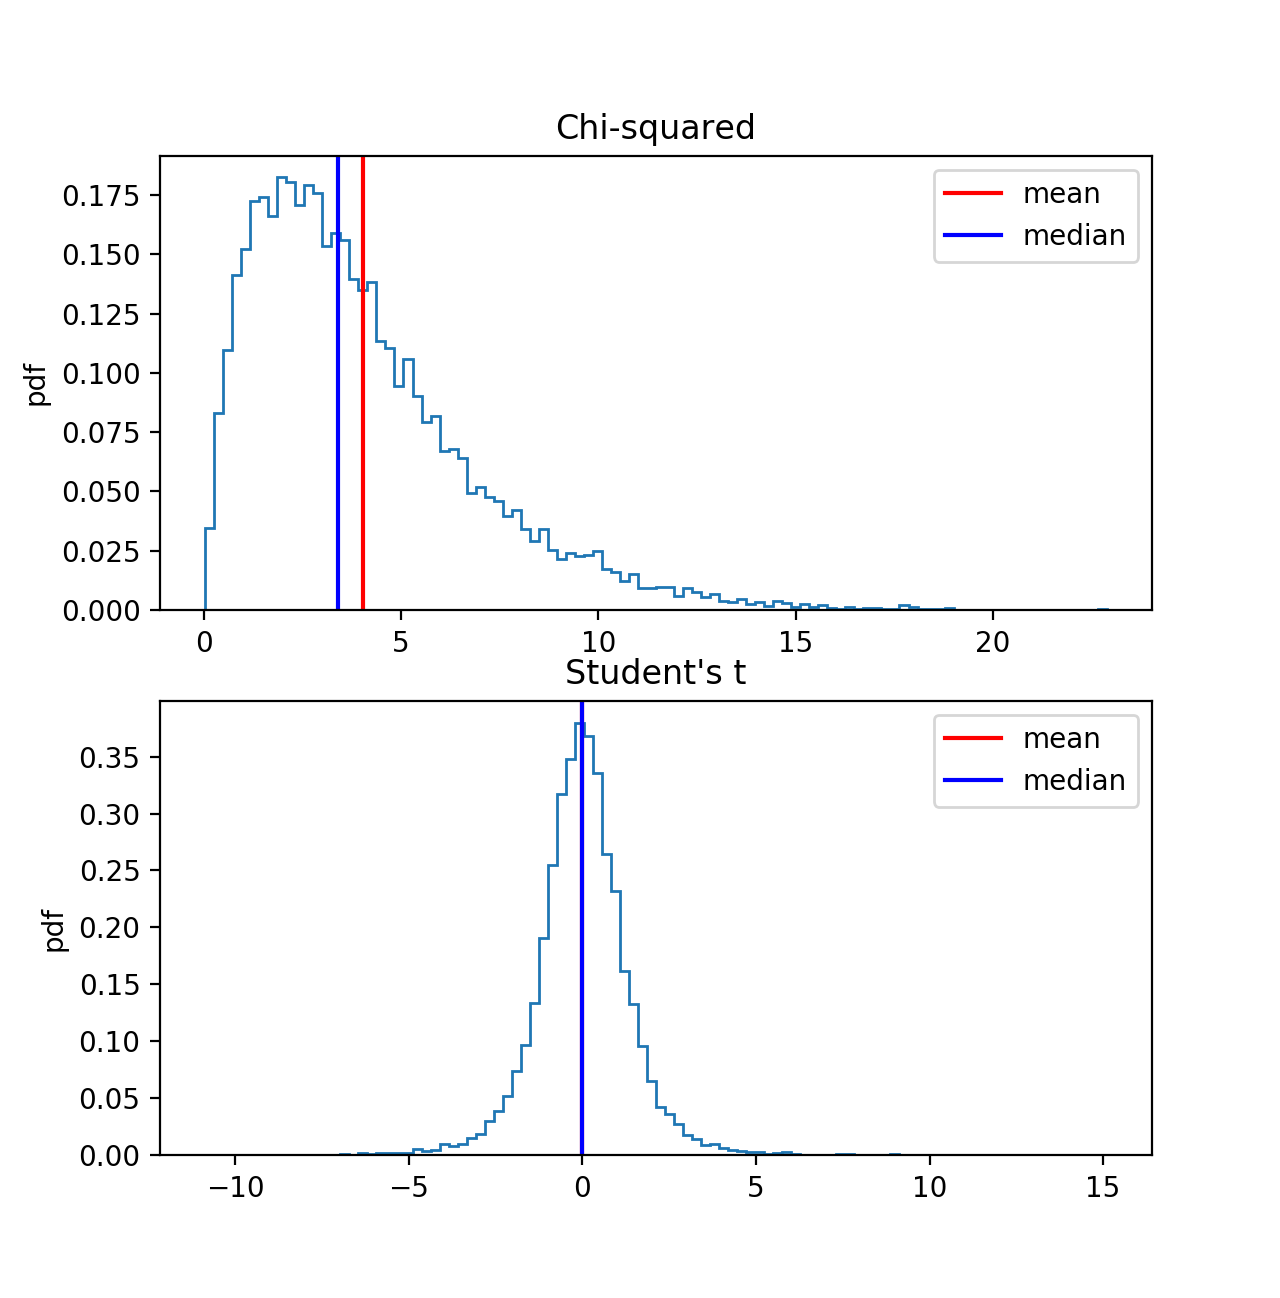
\includegraphics[width=\linewidth]{chi-sq_and_t_pdfs}
	\caption{Примеры асимметричного и heavy-tailed распределений (см. Таблицу~\ref{tbl:ex_pdfs}). Как можно наблюдать, для асимметричного распределения медиана -- более хороший эстиматор центральной тенденции, чем среднее; для симметричного распределения они совпадают в пределах погрешности.\label{fig:ex_pdfs}}
\end{figure}

\begin{table}
	\caption{Параметры распределений из Рис.~\ref{fig:ex_pdfs}\label{tbl:ex_pdfs}}
	\begin{tabular}{r|l|l|l|l}\hline
		Распределение & mean & median & skewness & kurtosis \\\hline
		$t$ & $9.54\cdot 10^{-3}$ & $1.65\cdot 10^{-2}$ & $8.31\cdot 10^{-2}$ & 8.07\\
		$\chi^2_4$ & 4.03 & 3.34 & 1.38 & 5.71 \\\hline
	\end{tabular}
\end{table}

\section{Доверительный интервал. Доверительная вероятность}
Предположим, вы измерили некоторую величину $X$ $n$ раз, и получили какую-то выборку $D = \{x_1, x_2, \dots x_n\}$. Построив гистограмму, вы решили, что  $X\sim N(\mu, \sigma)$. Теперь начальник требует от вас некоторую оценку величины $X$. Вы можете, конечно, дать ему значение $\avg{X} = M\left[X\right]$. Такая оценка будет называться \emph{точечной}. Более информативно будет дать что-то вроде $\avg{X} \pm \sigma_X$.

Так вот, интервал $I_{CI} = \left[\avg{X} - \sigma_X, \avg{X} + \sigma_X\right]$ называется \emph{доверительным интервалом} (confidence interval), а вероятность $p$ обнаружить очередное измерение $x_{n+1}$ внутри $I_{CI}$
называется \emph{доверительной вероятностью}. 
\begin{rmk}
	В рассматриваемом примере, кстати, доверительная вероятность будет 67\%.
\end{rmk}

\section{Двумерная случайная величина}
Если на пространстве событий $\Omega$ заданы \emph{две} случайные функции $X$ и $Y$, говорят, что задана \emph{двумерная} с.в.

Соответственно, кумулятивное распределение ${F_{X,Y}(x,y) = P(X<x\wedge Y<y)}$. Функция плотности распределения (joint probability density function) $f(x,y)$ определяется аналогично одномерному случаю.

\subsection{Ковариация и коэффициент корреляции}
В одномерном случае у нас был параметр дисперсии $\sigma_X$, такой, что вариация 
\begin{align*}
\var{X} = \sigma^2_X &= \avg{(X-\avg{X})^2} \\
 &= \avg{(X-\avg{X})(X-\avg{X})}.
\end{align*}

Акалогично, для двух с.в. можно определить ко-вариацию
\[
\cov{X, Y} = \sigma_{X,Y} = \avg{(X-\avg{X})(Y-\avg{Y})}.
\]
Иными словами
\[
\var{X} = \cov{X,X}.
\]
\emph{Коэффициент корреляции} -- это нормированная ковариация:
\[
\rho_{X,Y} = \frac{\sigma_{X,Y}}{\sigma_X\sigma_Y}.
\]
\section{Метод наименьших квадратов}
\subsection{Метод максимального правдоподобия}
Предположим, мы измерили некоторую с.в. $X\sim f(\vec \theta)$ несколько раз, получили набор значений $\{x_1, x_2,\dots,x_n\}$, и теперь хотим определить значения параметров $\vec\theta = (\theta_1, \theta_2, \dots)$.~\footnote{Именно эта задача возникает, когда мы пытаемся профитировать данные какой-то функцией.}

Это можно сделать методом максимального правдоподобия, который заключается в следующем:
\begin{enumerate}
	\item Cоставляем функцию правдоподобия $L(\vec\theta|\vec x) = f(\vec x|\vec\theta)$.~\footnote{По сути, функция правдоподобия -- это вероятность наблюдения данного набора данных, при данном значении параметра; но интрпретируется как функция $\vec\theta$, а данные считаются параметром.}
	\item  Пытаемся подобрать вектор параметров $\vec\theta_0$, который бы максимизировал $L(\vec\theta|\vec x)$.
\end{enumerate}

\begin{rmk}[independent identically distributed]
	Поскольку в нашей задаче рассматриваются отдельные измерения одной и той же величины, логично предположить, что $x_{i+1}$ независимо от $x_i$, и что все измерения происходят из одного и того же распределения. Тогда 
	\[
	L(\vec\theta|\vec x) = f(\vec x|\vec\theta) = \prod_{i=1}^n f(x_i|\vec\theta).
	\]
\end{rmk}

\subsection{Статистика $\chi^2$}
Сделаем \emph{ещё одно} предположение: пускай 
\begin{align*}
f(x_i|\vec\theta) &= f(x_i|(\mu,\sigma)) \\
&= \frac{1}{\sqrt{2\pi}\sigma}\cdot \exp\left[-\frac12\left(\frac{x_i-\mu}{\sigma}\right)^2\right].
\end{align*}

В таком случае, удобнее не \emph{максимизировать} $L(\vec\theta|\vec x)$, а \emph{минимизировать} функцию $-\ln L(\vec\theta|\vec x)$:
\begin{align*}
	-\ln L(\vec\theta|\vec x) &= -\ln\left(\prod_i f(x_i|\vec\theta)\right) \\
	&= -\ln\left[K_1\cdot  \exp\left(-\frac12\sum_i \left(\frac{x_i-\mu}{\sigma}\right)^2\right)\right] \\
	&= \ln K + \frac12\sum_i\left(\frac{x_i-\mu}{\sigma}\right)^2.
\end{align*}

Иными словами, нужно \emph{минимизировать сумму квадратов} отклонений измерений от ожидания
\[
\sum_i\left(\frac{x_i-\mu}{\sigma}\right)^2.
\]

\begin{rmk}[Наконец-то $\chi^2$]
	Пусть у нас есть набор с.в.  $X_i\sim N(\mu, \sigma)$; тогда с.в.
	\begin{align}
	Y_i &= \frac{X_i-\mu}{\sigma} \sim N(0,1),
	\intertext{а сумма}
	Z &= \sum_{i=1}^{n} Y_i^2 \sim \chi^2_n
	\end{align}
\end{rmk}
\end{document}